\documentclass[11pt]{article}
\usepackage[margin=0.9in]{geometry}
\usepackage{amsmath,amssymb}
\usepackage{booktabs}
\usepackage{graphicx}
\usepackage{listings}
\usepackage{xcolor}
\usepackage[hidelinks]{hyperref}
\newcommand{\code}[1]{\texttt{#1}}

% notebook-style boxes: code cells (light gray) and output cells (framed)
\definecolor{cellbg}{RGB}{247,247,247}
\definecolor{outbg}{RGB}{255,255,255}
\lstdefinestyle{pycode}{language=Python, basicstyle=\ttfamily\scriptsize,
  backgroundcolor=\color{cellbg}, frame=single, rulecolor=\color{black!25},
  showstringspaces=false, breaklines=true, columns=fullflexible,
  keepspaces=true, commentstyle=\color{black!55},
  keywordstyle=\color{blue!60!black}, stringstyle=\color{green!40!black},
  numbers=left, numberstyle=\tiny\color{black!40}, xleftmargin=1.6em}
\lstdefinestyle{out}{basicstyle=\ttfamily\scriptsize,
  backgroundcolor=\color{outbg}, frame=single, rulecolor=\color{black!45},
  breaklines=true, columns=fullflexible, keepspaces=true}

\title{OpenSG-RM Plate: Tutorials\\[4pt]
\large Four standalone, fully runnable cases with their real outputs}
\author{OpenSG-TW}
\date{\today}

\begin{document}
\maketitle

Each tutorial is a \textbf{complete standalone script} committed at
\code{docs/rm\_plate\_manual/tutorial\_caseN.py}.  Run it from anywhere
inside the repository with no edits and no further involvement:
\begin{lstlisting}[style=out]
python docs/rm_plate_manual/tutorial_case1.py
\end{lstlisting}
Every script: builds its 1-D SG YAML and mesh figure, homogenizes and
\emph{prints the plate law}, computes the plate solution of its benchmark
problem, dehomogenizes the full 3-D stress and displacement fields at the two
governing stations, compares against the exact 3-D elasticity solution of
the same problem, writes the out-of-plane / in-plane / displacement figures,
and evaluates \emph{both} the max-stress and Tsai--Wu failure indices from
the recovered ply-frame stresses.  The output blocks and figures below are
the \emph{actual} products of running the scripts.

\paragraph{User options (every tutorial).}
\begin{lstlisting}[style=out]
--model 0     classical ABD: 6x6 lamination matrix, Kirchhoff kinematics
--model 1     RM shear-refined 8x8 (default)
--FF N11 N22 N12 M11 M22 M12 Q1 Q2
              dehomogenize from YOUR resultants (the exact-3-D comparison
              is skipped: an arbitrary FF has no exact twin)
\end{lstlisting}

\tableofcontents

%=====================================================================
\newpage
\section{Tutorial 1: cross-ply [0/90/0], $S=a/h=10$}
Simply supported strip, span $a=1$~m, thickness $h=a/10$, top-face pressure
$q(x)=q_0\sin(\pi x/a)$ with $q_0=10$~kPa; graphite/epoxy 25:1 plies, three
equal thicknesses, $[0/90/0]$ bottom-up, mid-surface reference.

\begin{figure}[htb]\centering
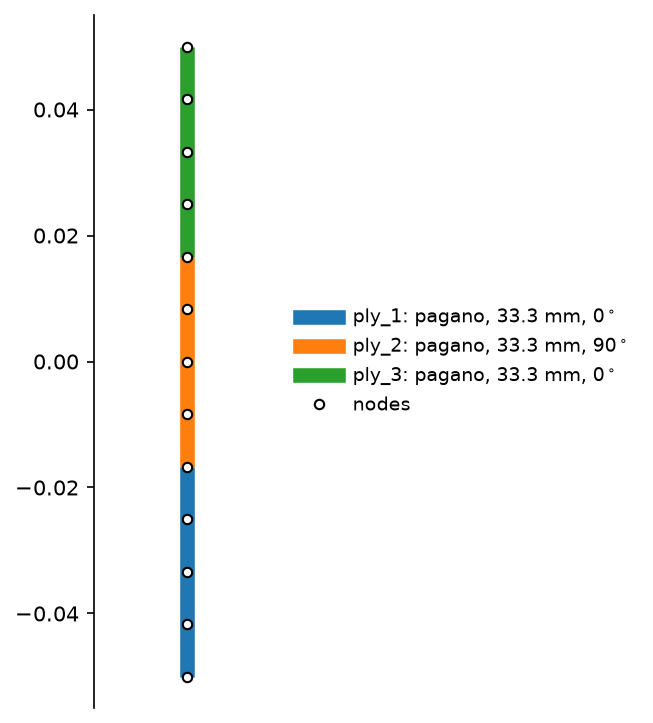
\includegraphics[width=0.55\textwidth]{tutorial_case1_sg.png}
\caption{The 1-D through-thickness SG of Tutorial 1 (three plies, one
element each), as written by the script.}
\end{figure}

\subsection{The complete script}
\lstinputlisting[style=pycode]{tutorial_case1.py}

\subsection{Output of the default run}
\lstinputlisting[style=out]{tutorial_case1_output.txt}

\subsection{Results}
\begin{figure}[htb]\centering
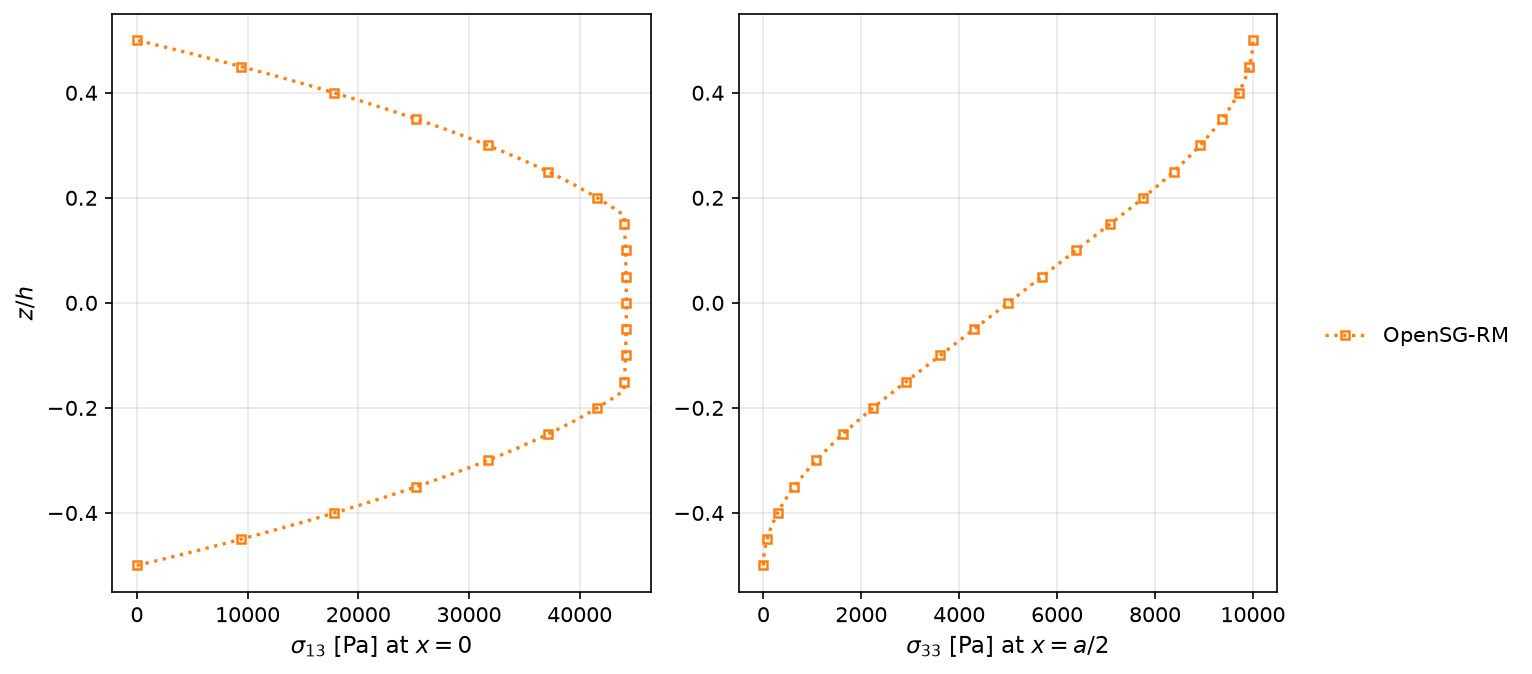
\includegraphics[width=0.78\textwidth]{tutorial_case1_outofplane.png}
\caption{Out-of-plane stresses, OpenSG-RM vs the exact 3-D solution.}
\end{figure}
\begin{figure}[htb]\centering
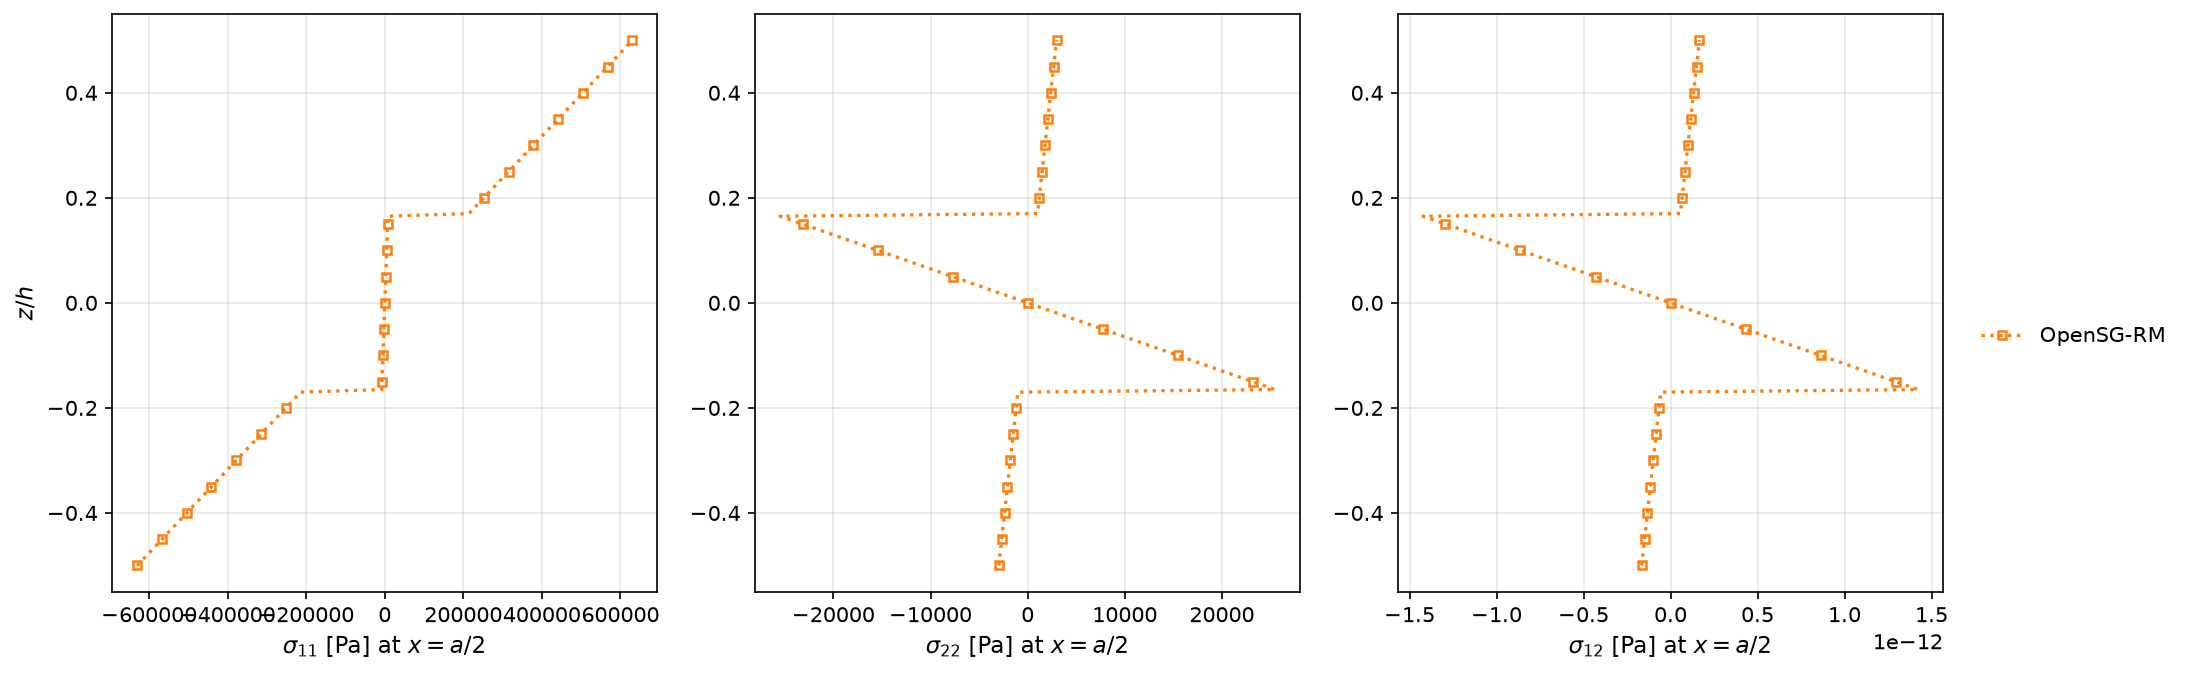
\includegraphics[width=0.98\textwidth]{tutorial_case1_inplane.png}
\caption{In-plane stresses at the bending peak.}
\end{figure}
\begin{figure}[htb]\centering
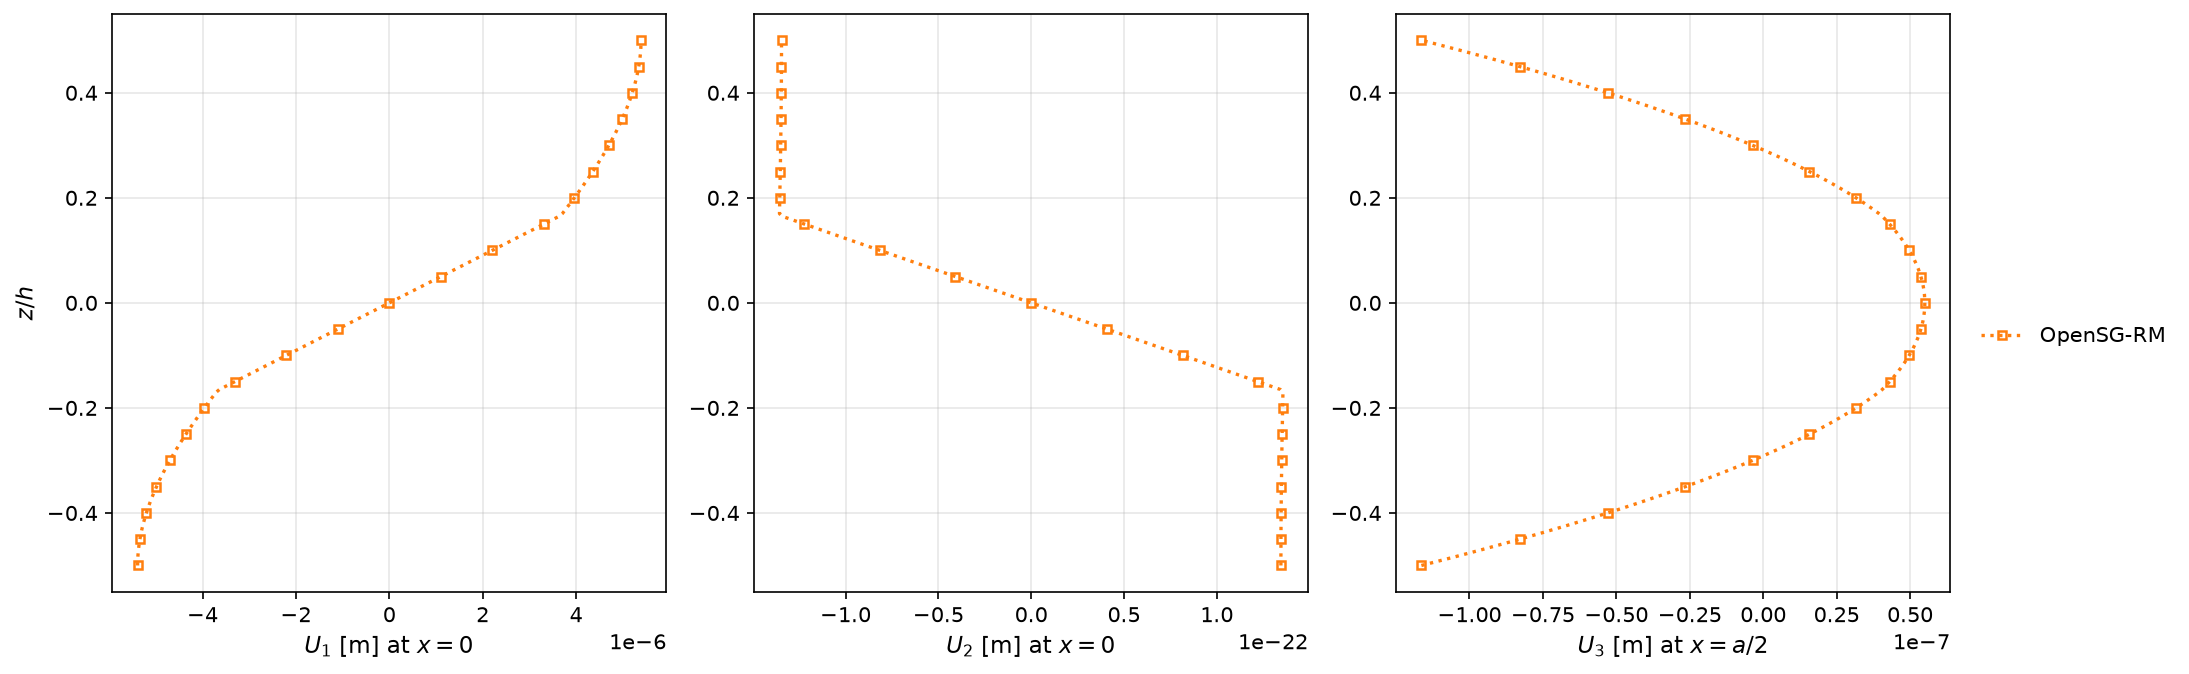
\includegraphics[width=0.98\textwidth]{tutorial_case1_disp.png}
\caption{Recovered 3-D displacements.}
\end{figure}

\clearpage
\subsection{Using the options}
\textbf{Classical ABD (\code{--model 0}).}  Same script, classical
lamination matrix and Kirchhoff kinematics --- the errors show exactly what
the shear refinement buys at $S=10$:
\lstinputlisting[style=out]{tutorial_case1_model0_output.txt}

\textbf{User resultants (\code{--FF}).}  Dehomogenization from a
user-supplied resultant vector (here the strip's own statics values
$M_{11}=q_0/p^2$, $Q_1=q_0/p$, so the recovered fields reproduce the
default run's shear station):
\lstinputlisting[style=out]{tutorial_case1_ff_output.txt}

%=====================================================================
\newpage
\section{Tutorial 2: sandwich [0/core/0], $S=10$}
Same strip and load as Tutorial 1; stiff carbon faces ($0.1h$ each) over a
soft core ($0.8h$) --- the layup where the soft core makes transverse shear
dominant.  Only the material/layup block differs from Tutorial~1.

\begin{figure}[htb]\centering
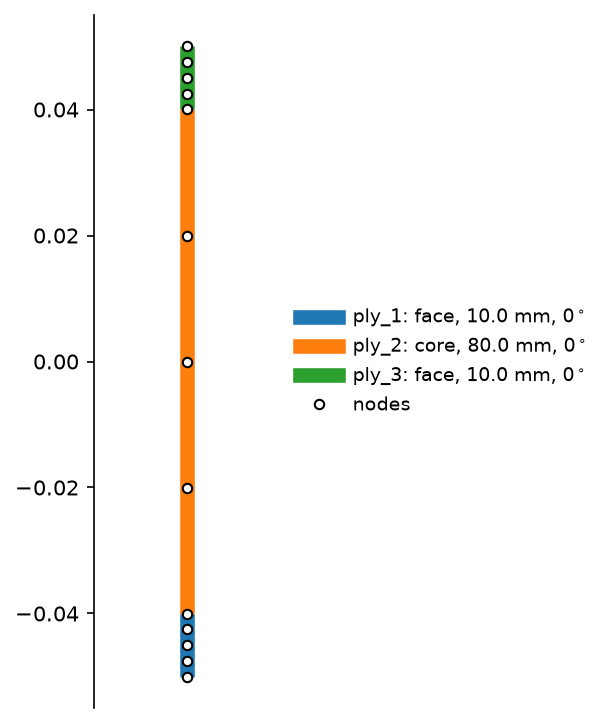
\includegraphics[width=0.55\textwidth]{tutorial_case2_sg.png}
\caption{The 1-D SG of Tutorial 2 (face/core/face).}
\end{figure}

\subsection{The complete script}
\lstinputlisting[style=pycode]{tutorial_case2.py}

\subsection{Output of the default run}
\lstinputlisting[style=out]{tutorial_case2_output.txt}

\subsection{Results}
\begin{figure}[htb]\centering
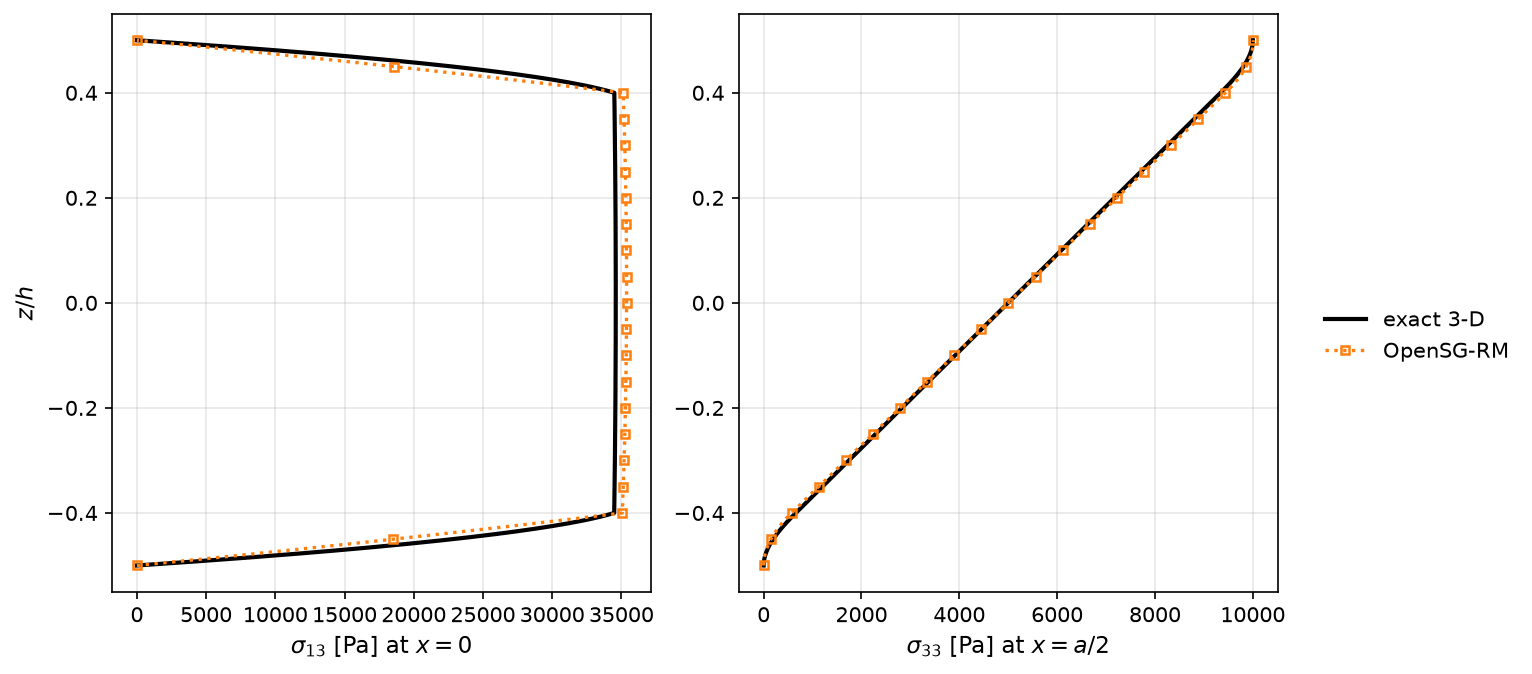
\includegraphics[width=0.78\textwidth]{tutorial_case2_outofplane.png}
\caption{Out-of-plane stresses: the transverse shear lives almost entirely
in the soft core; $\sigma_{33}$ from the equilibrium route.}
\end{figure}
\begin{figure}[htb]\centering
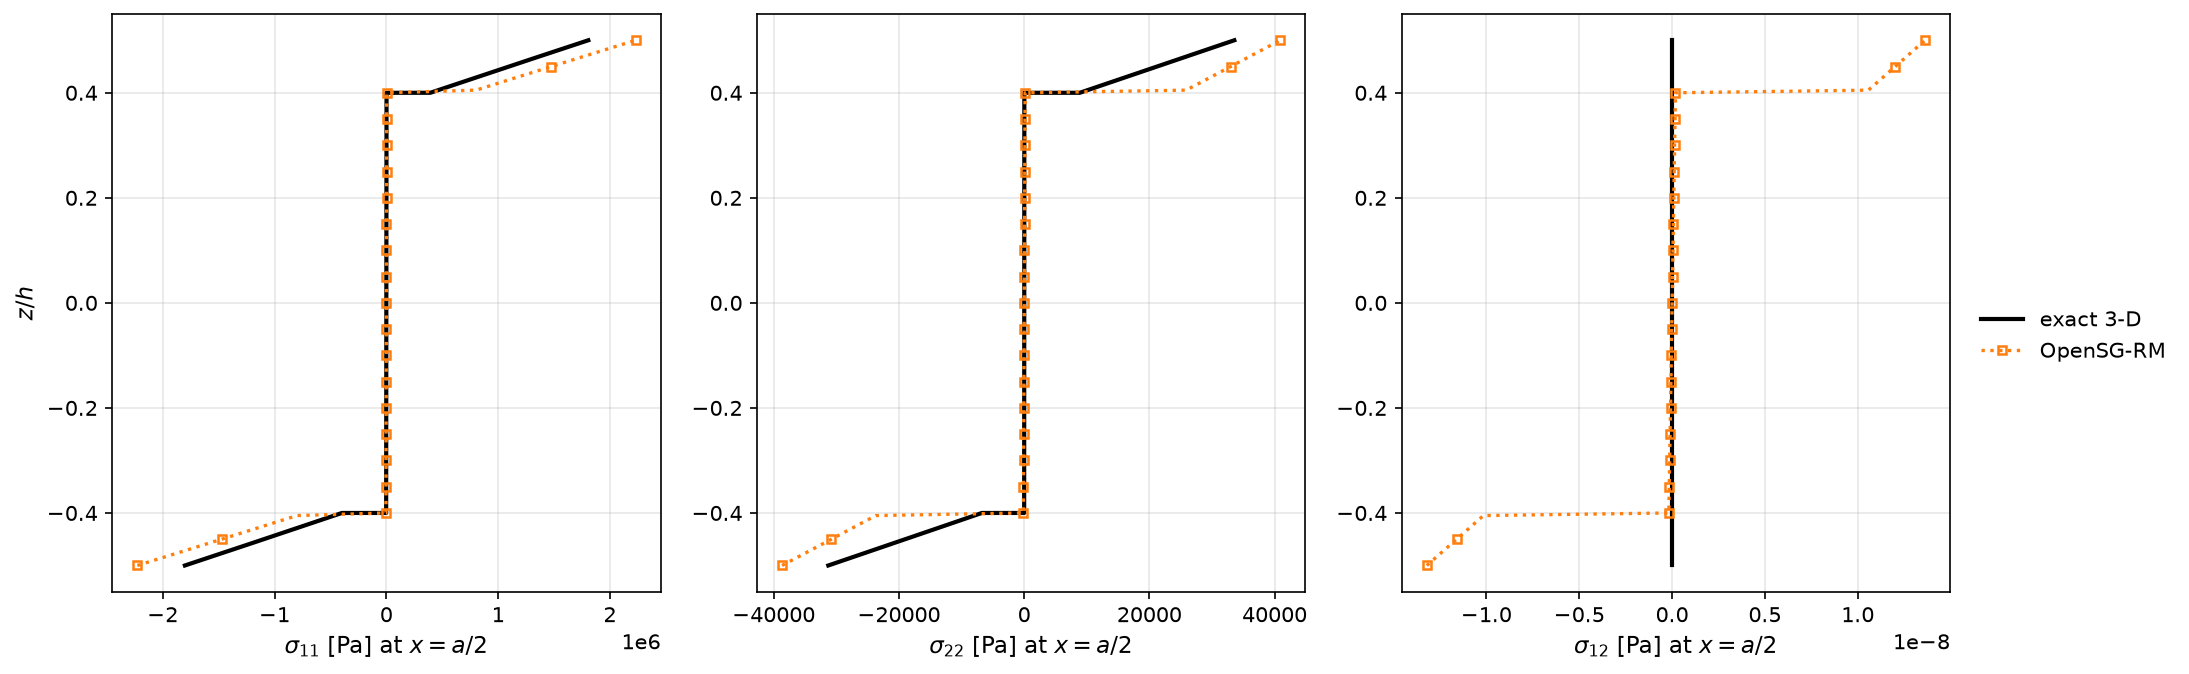
\includegraphics[width=0.98\textwidth]{tutorial_case2_inplane.png}
\caption{In-plane stresses.  At $S=10$ the soft-core in-plane recovery is
regime-limited (the errors collapse to 1--3\,\% by $S=50$); the transverse
components and displacements above remain accurate.}
\end{figure}
\begin{figure}[htb]\centering
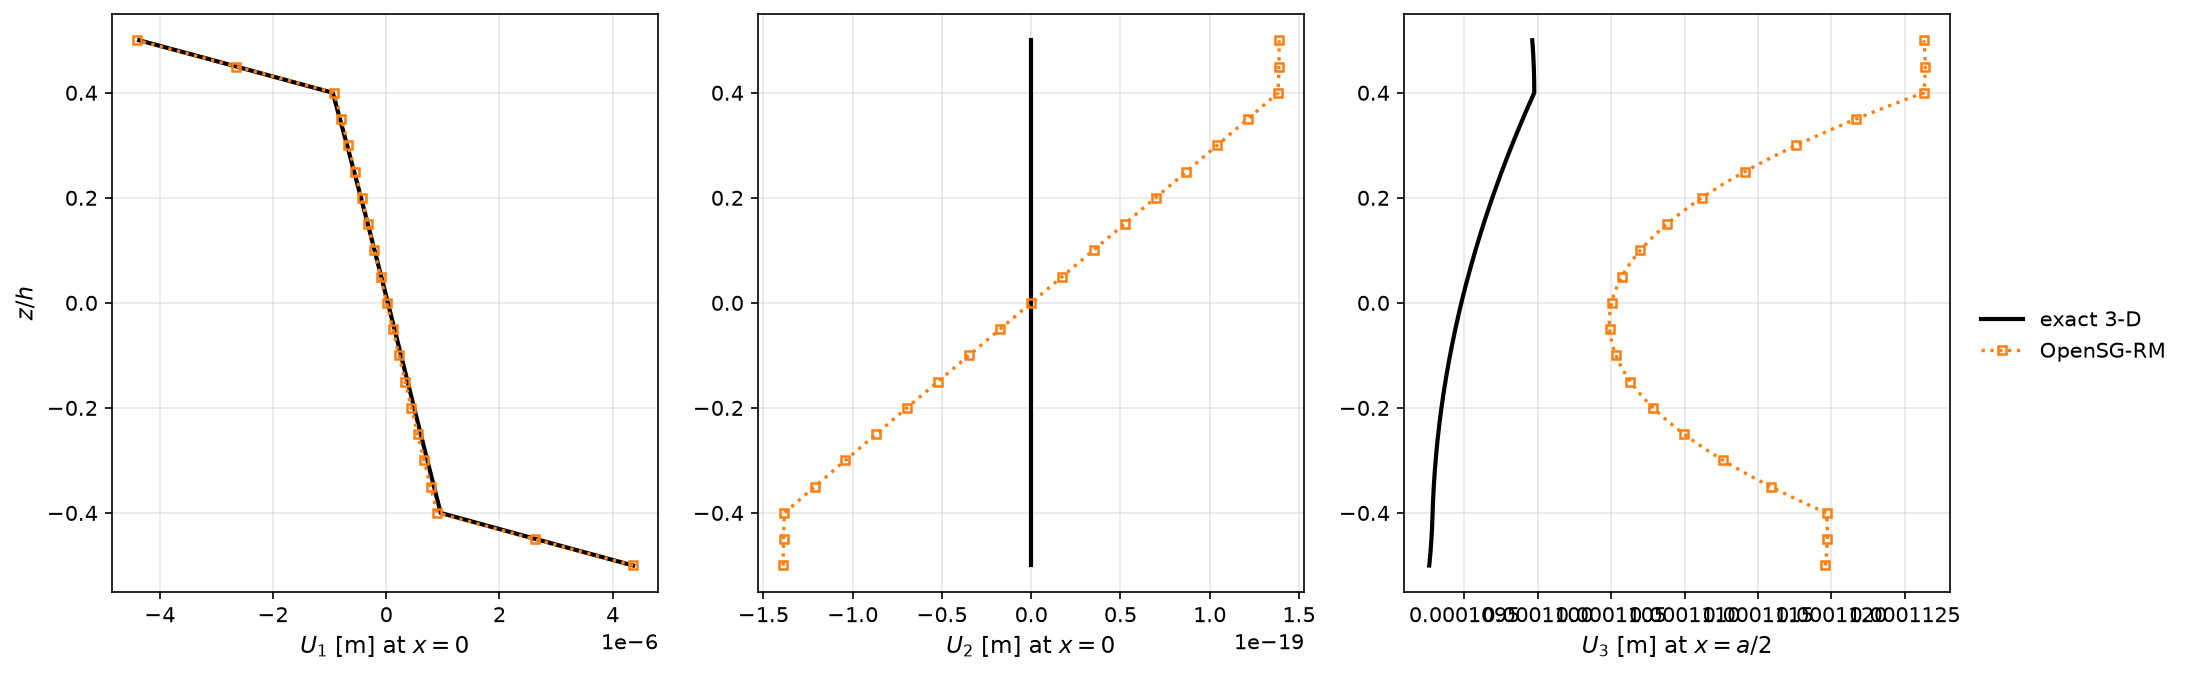
\includegraphics[width=0.98\textwidth]{tutorial_case2_disp.png}
\caption{Recovered 3-D displacements.}
\end{figure}

%=====================================================================
\newpage
\section{Tutorial 3: antisymmetric angle ply [15/$-$15], $L/h=4$}
A deliberately \emph{thick} plate: span $a=4$~in, thickness $h=1$~in, loaded
on \emph{both} faces, $\sigma_{33}=\pm(q_0/2)\sin(\pi x/a)$ with
$q_0=1$~psi; two equal plies $[15/-15]$ bottom-up (25:1 material, psi--in
units).  The off-axis plies couple: the plate solution carries nonzero
$N_{22},M_{22},M_{12},Q_2$ and the response has $\sigma_{23}$ and $U_2$ ---
all recovered.

\begin{figure}[htb]\centering
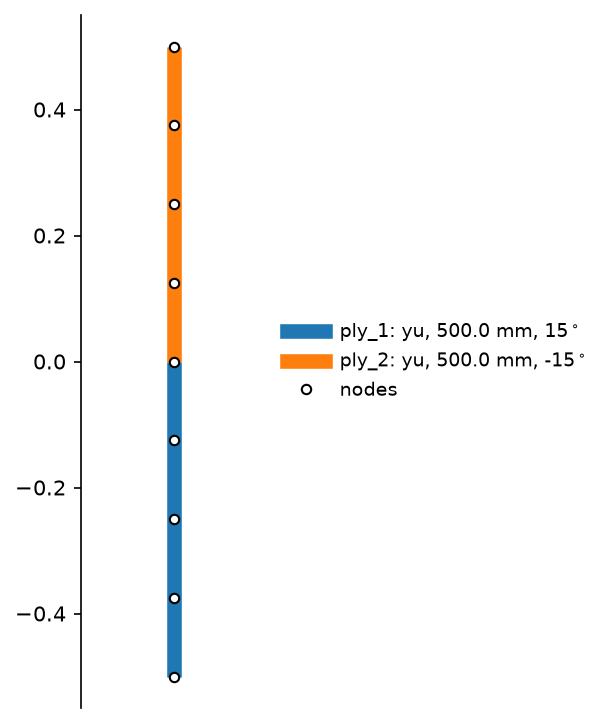
\includegraphics[width=0.55\textwidth]{tutorial_case3_sg.png}
\caption{The 1-D SG of Tutorial 3 (two plies).}
\end{figure}

\subsection{The complete script}
\lstinputlisting[style=pycode]{tutorial_case3.py}

\subsection{Output of the default run}
\lstinputlisting[style=out]{tutorial_case3_output.txt}

\subsection{Results}
\begin{figure}[htb]\centering
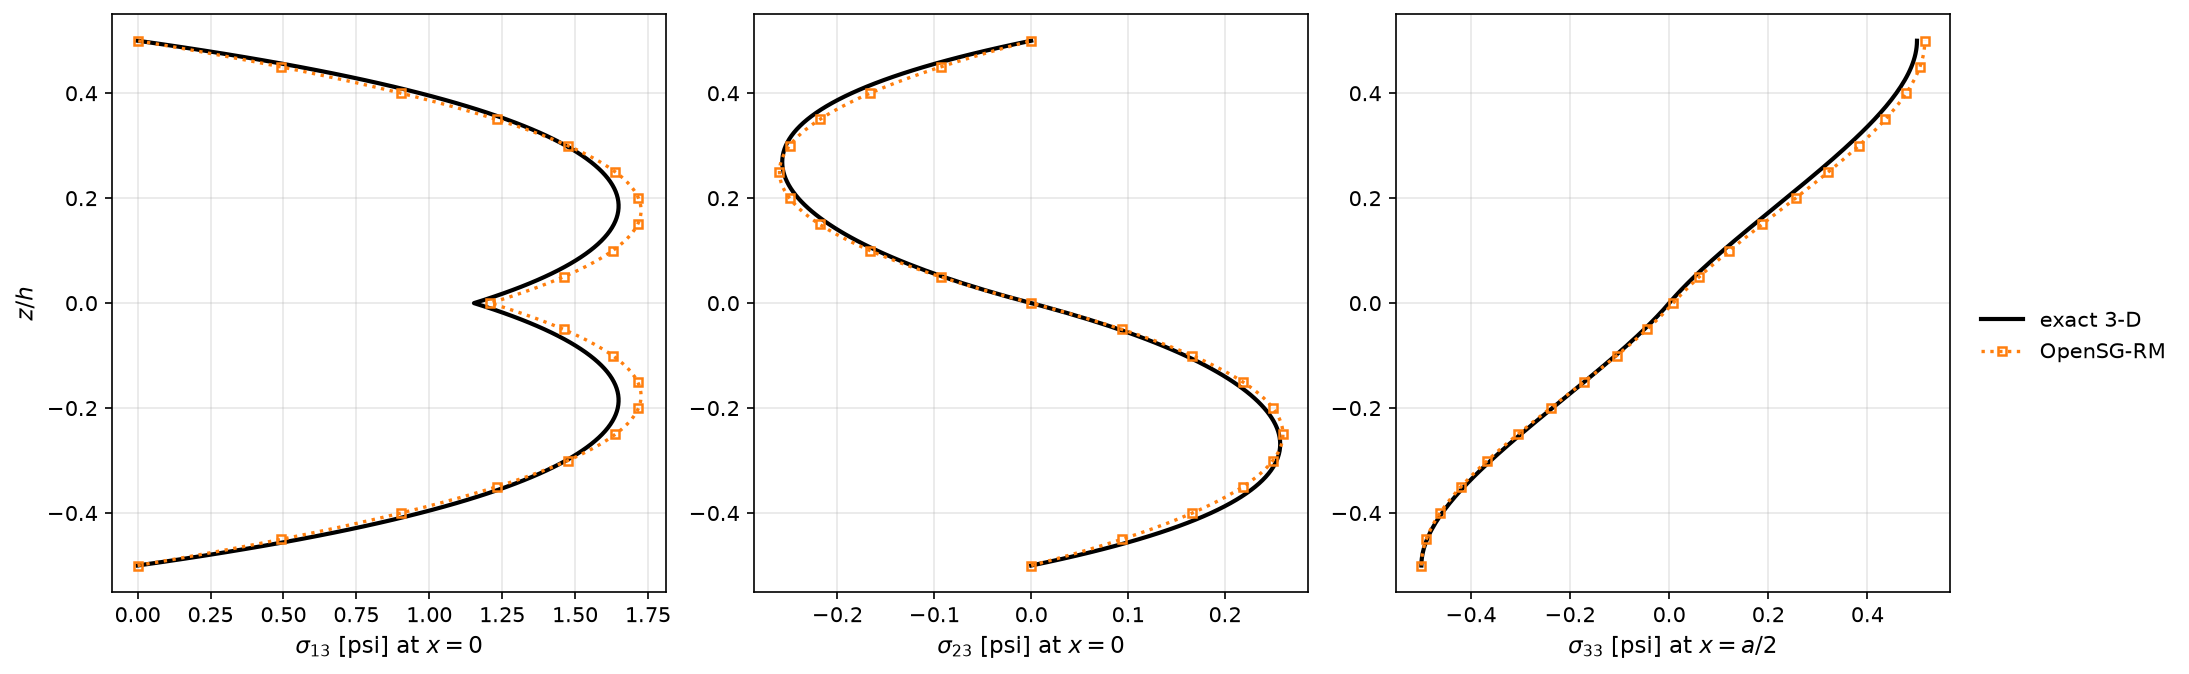
\includegraphics[width=0.98\textwidth]{tutorial_case3_outofplane.png}
\caption{Out-of-plane stresses at $L/h=4$; the split face load makes the
$\sigma_{33}$ faces $\pm q_0/2$.}
\end{figure}
\begin{figure}[htb]\centering
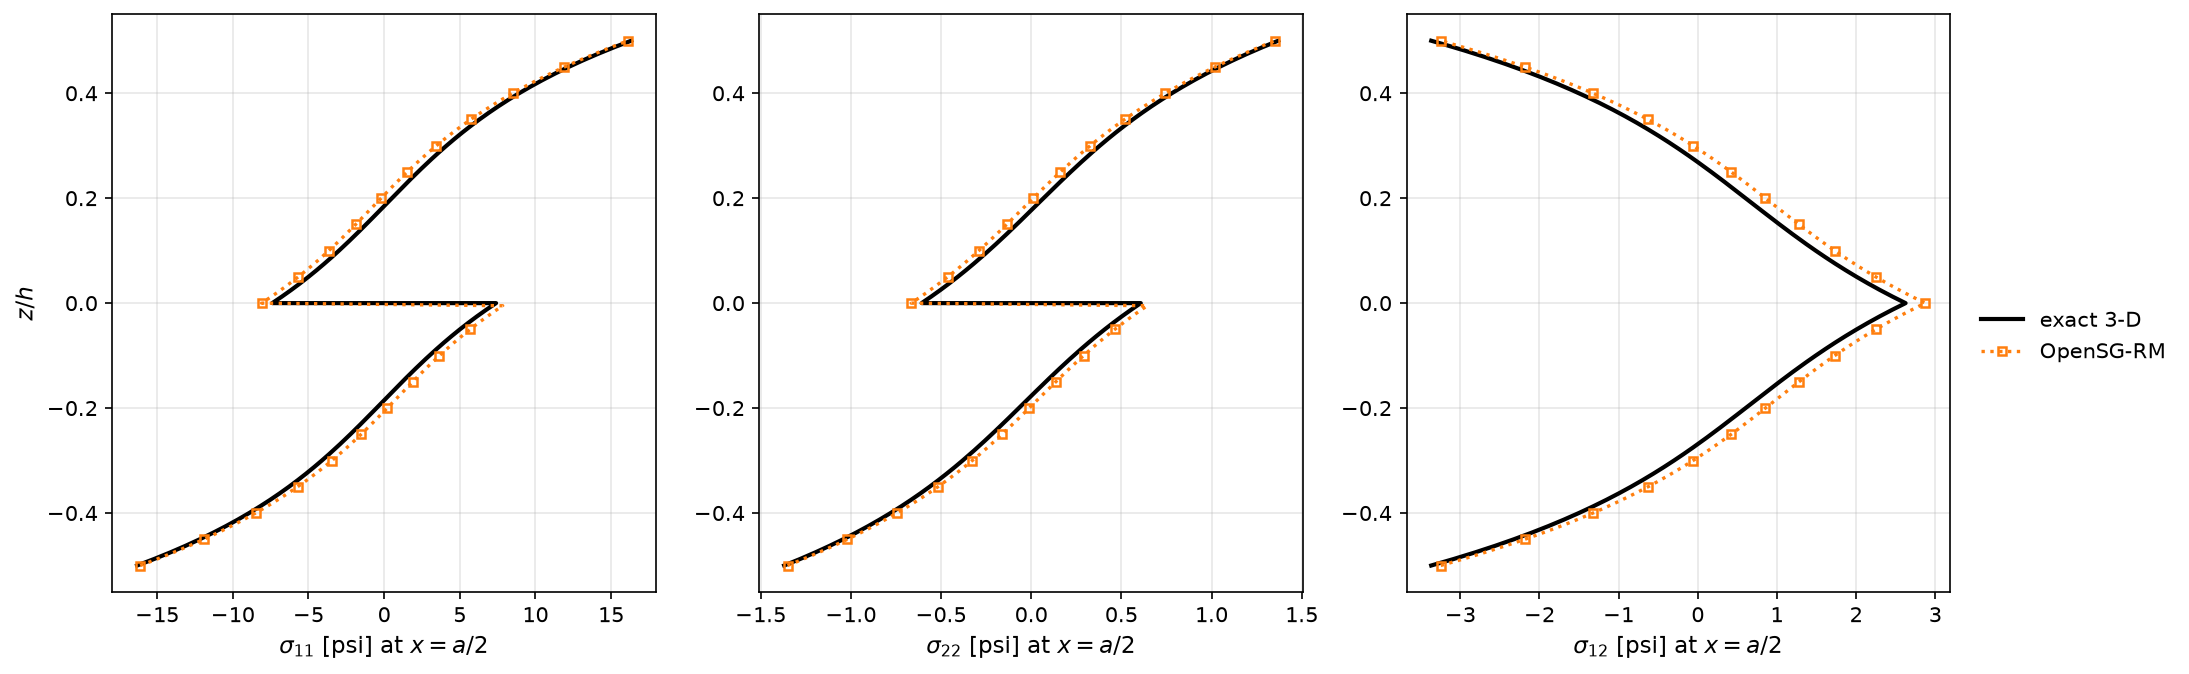
\includegraphics[width=0.98\textwidth]{tutorial_case3_inplane.png}
\caption{In-plane stresses --- $\sigma_{12}$ is a genuine field for the
angle plies.}
\end{figure}
\begin{figure}[htb]\centering
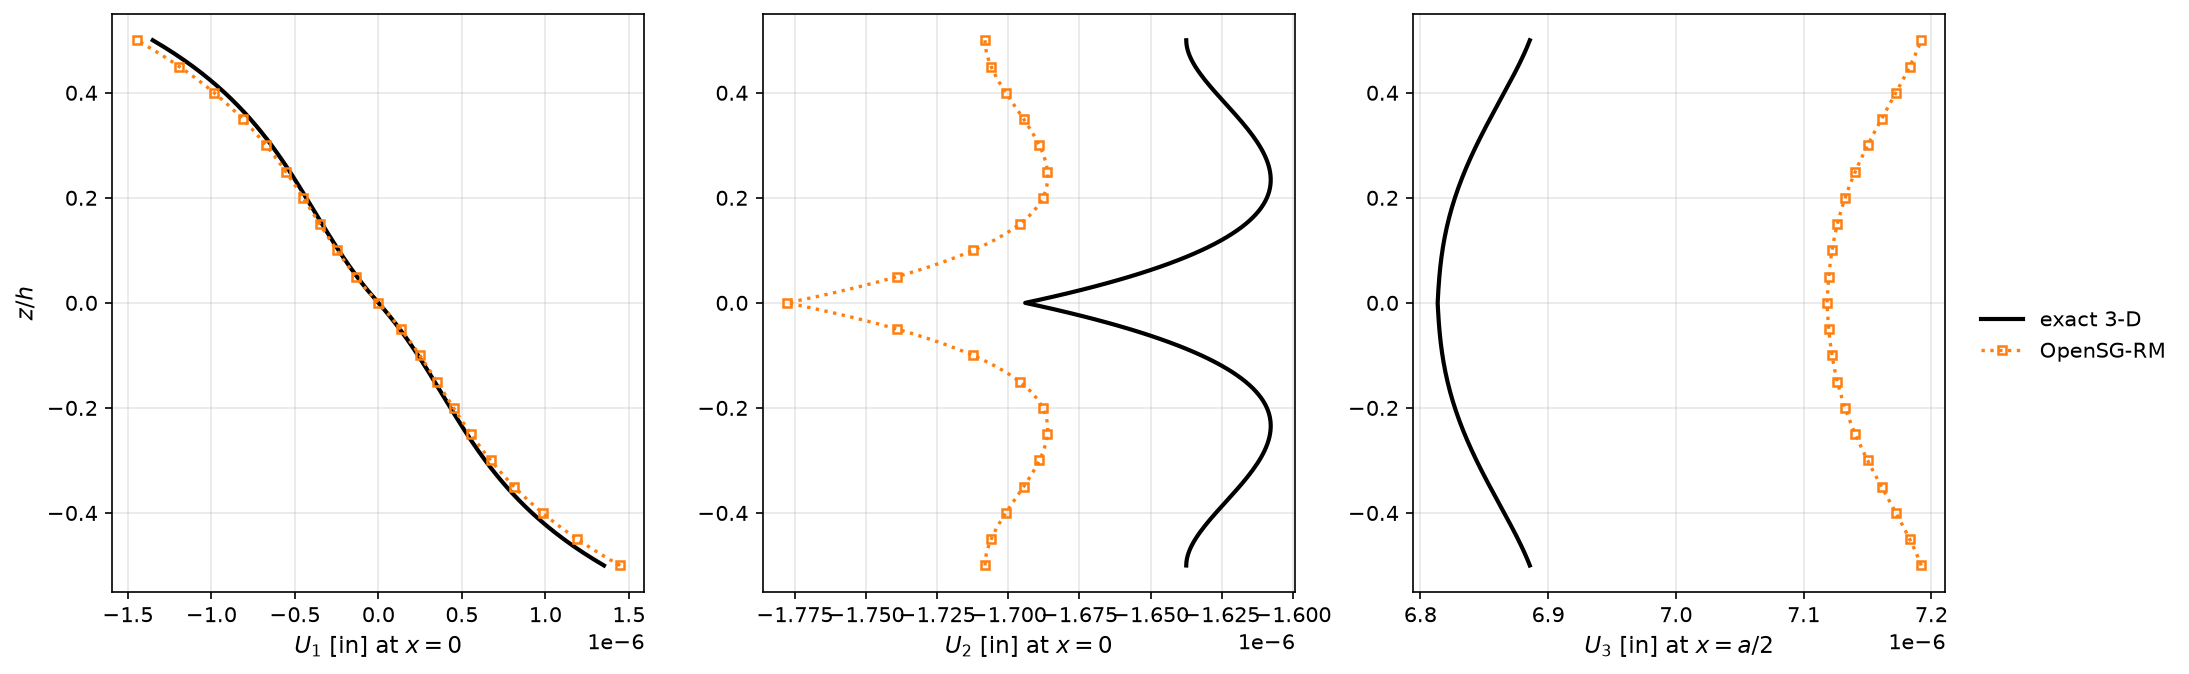
\includegraphics[width=0.98\textwidth]{tutorial_case3_disp.png}
\caption{Recovered 3-D displacements, including the coupled $U_2$.}
\end{figure}

%=====================================================================
\newpage
\section{Tutorial 4: symmetric angle ply [30/$-$30/$-$30/30], $L/h=4$}
Same geometry, material and split load as Tutorial 3; four equal plies
$[30/-30/-30/30]$.  $B=0$ (symmetric) but the bending--twist coupling makes
$M_{12}$, $Q_2$ and $\sigma_{23}$ large ($\sigma_{23}\sim0.5\,q_0$).

\begin{figure}[htb]\centering
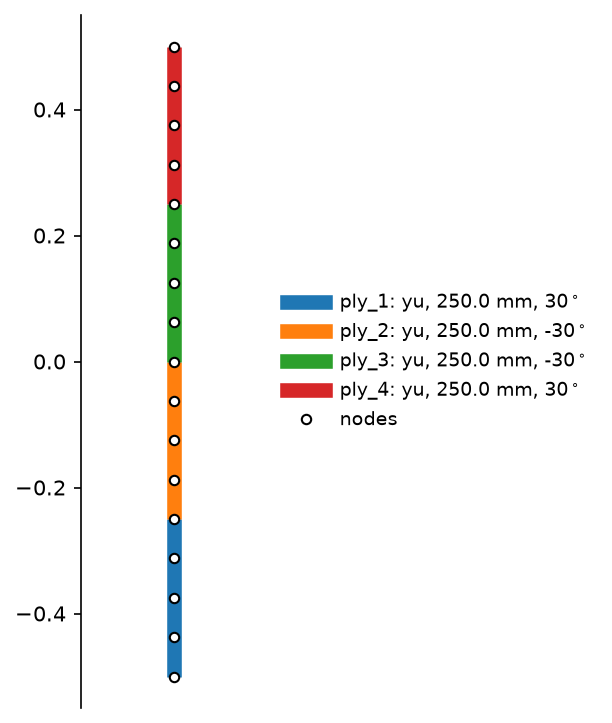
\includegraphics[width=0.55\textwidth]{tutorial_case4_sg.png}
\caption{The 1-D SG of Tutorial 4 (four plies).}
\end{figure}

\subsection{The complete script}
\lstinputlisting[style=pycode]{tutorial_case4.py}

\subsection{Output of the default run}
\lstinputlisting[style=out]{tutorial_case4_output.txt}

\subsection{Results}
\begin{figure}[htb]\centering
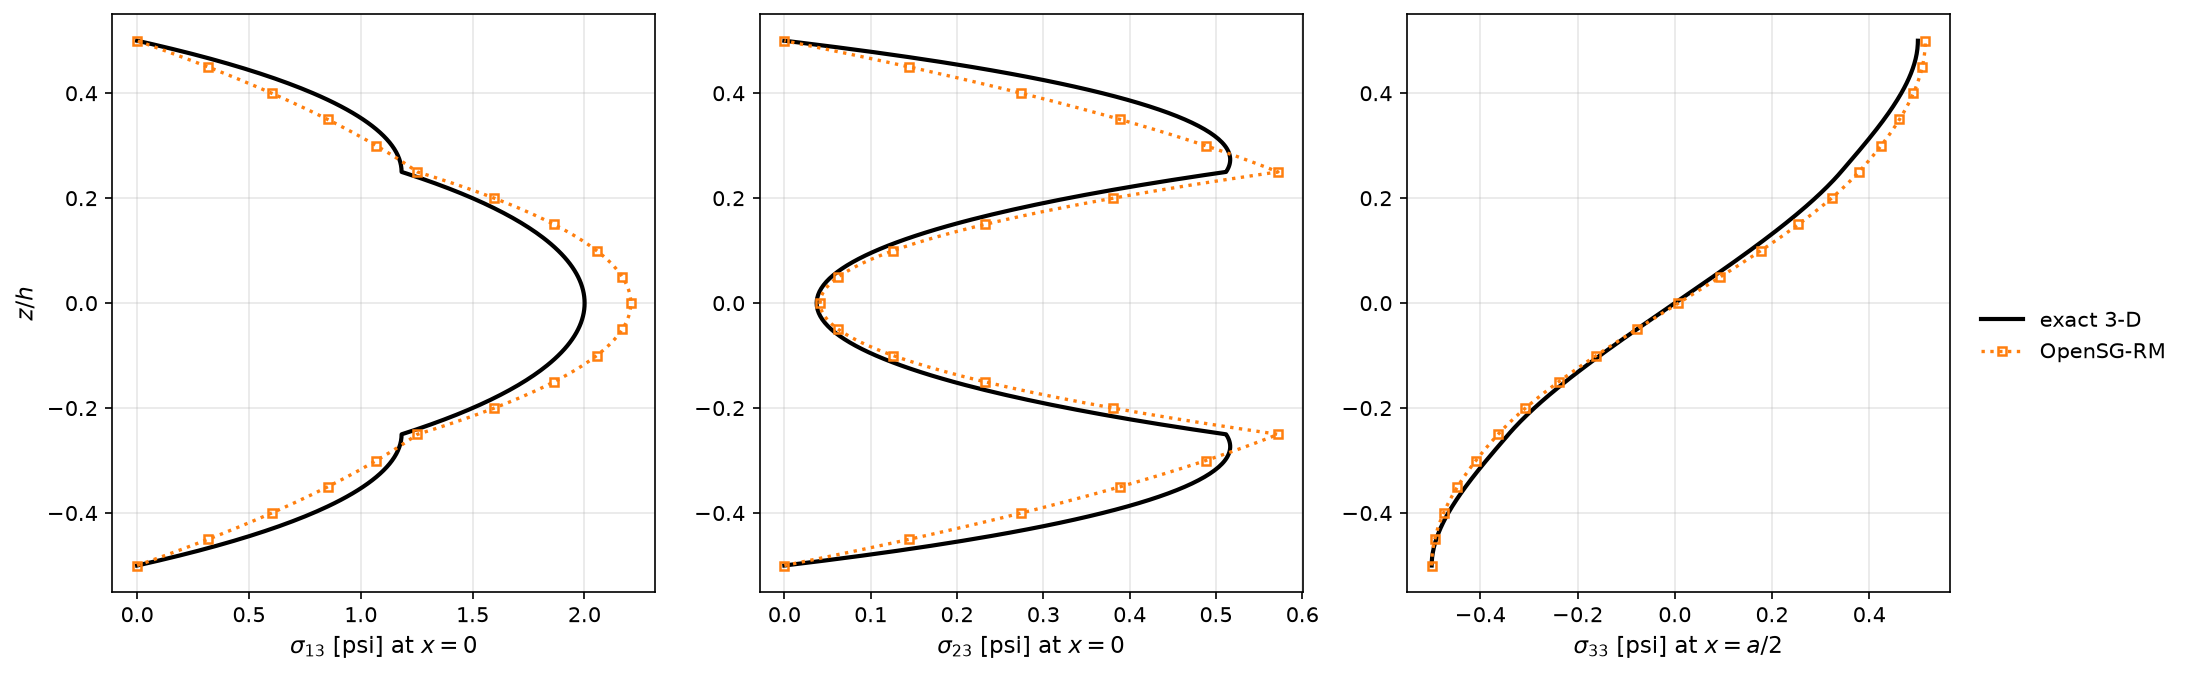
\includegraphics[width=0.98\textwidth]{tutorial_case4_outofplane.png}
\caption{Out-of-plane stresses; the strongest $\sigma_{23}$ of the four
cases.}
\end{figure}
\begin{figure}[htb]\centering
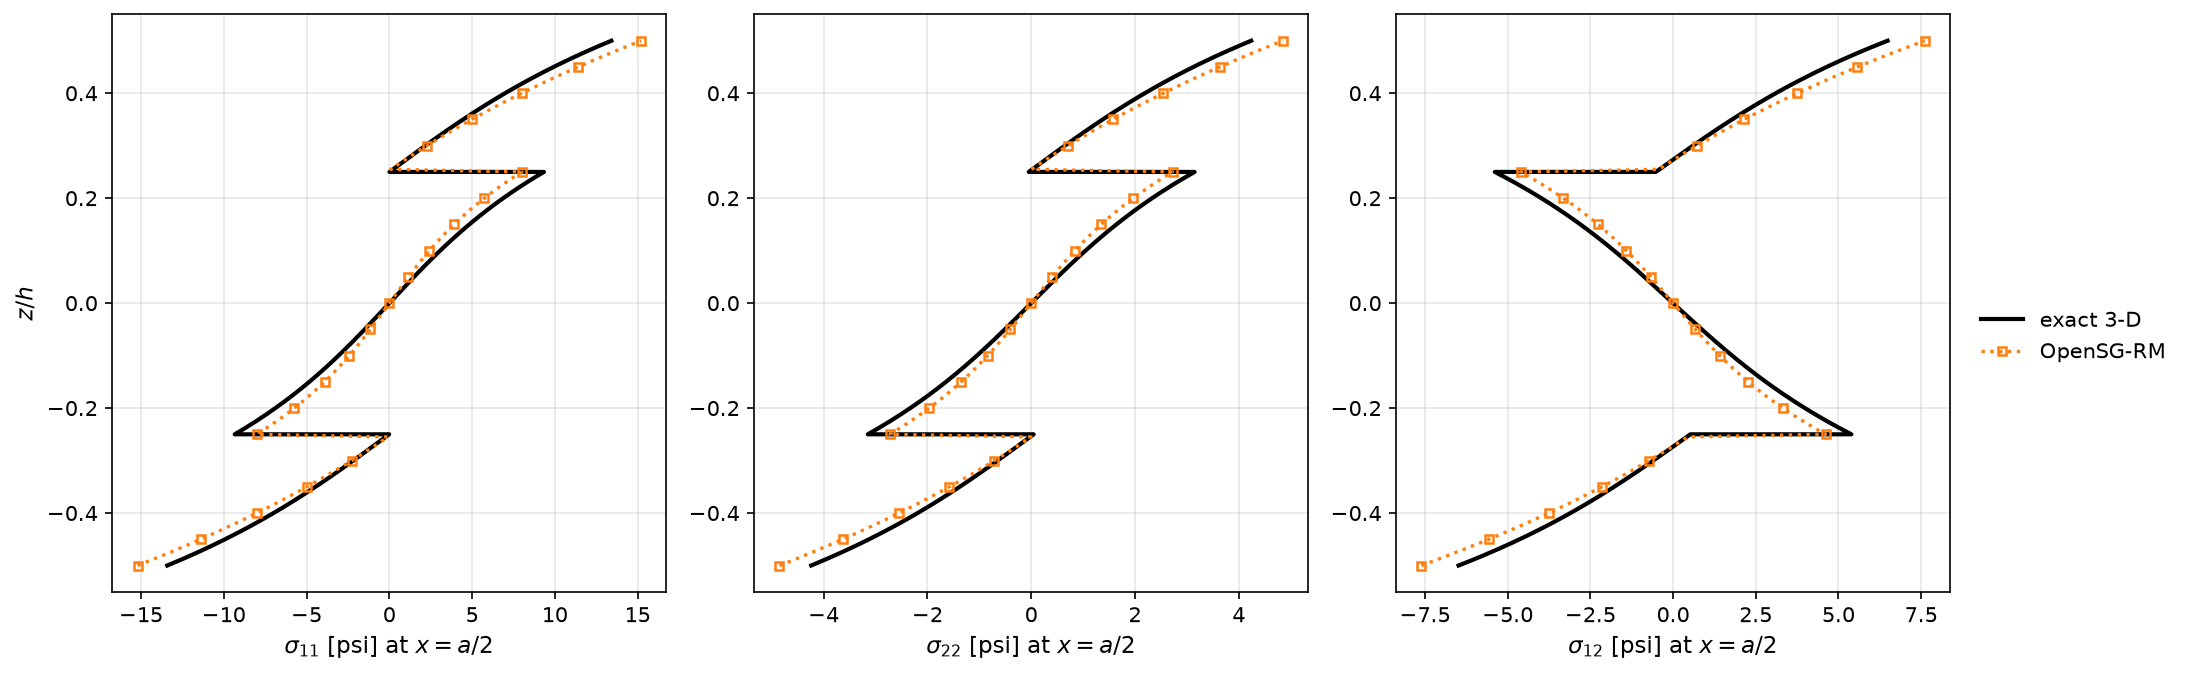
\includegraphics[width=0.98\textwidth]{tutorial_case4_inplane.png}
\caption{In-plane stresses.}
\end{figure}
\begin{figure}[htb]\centering
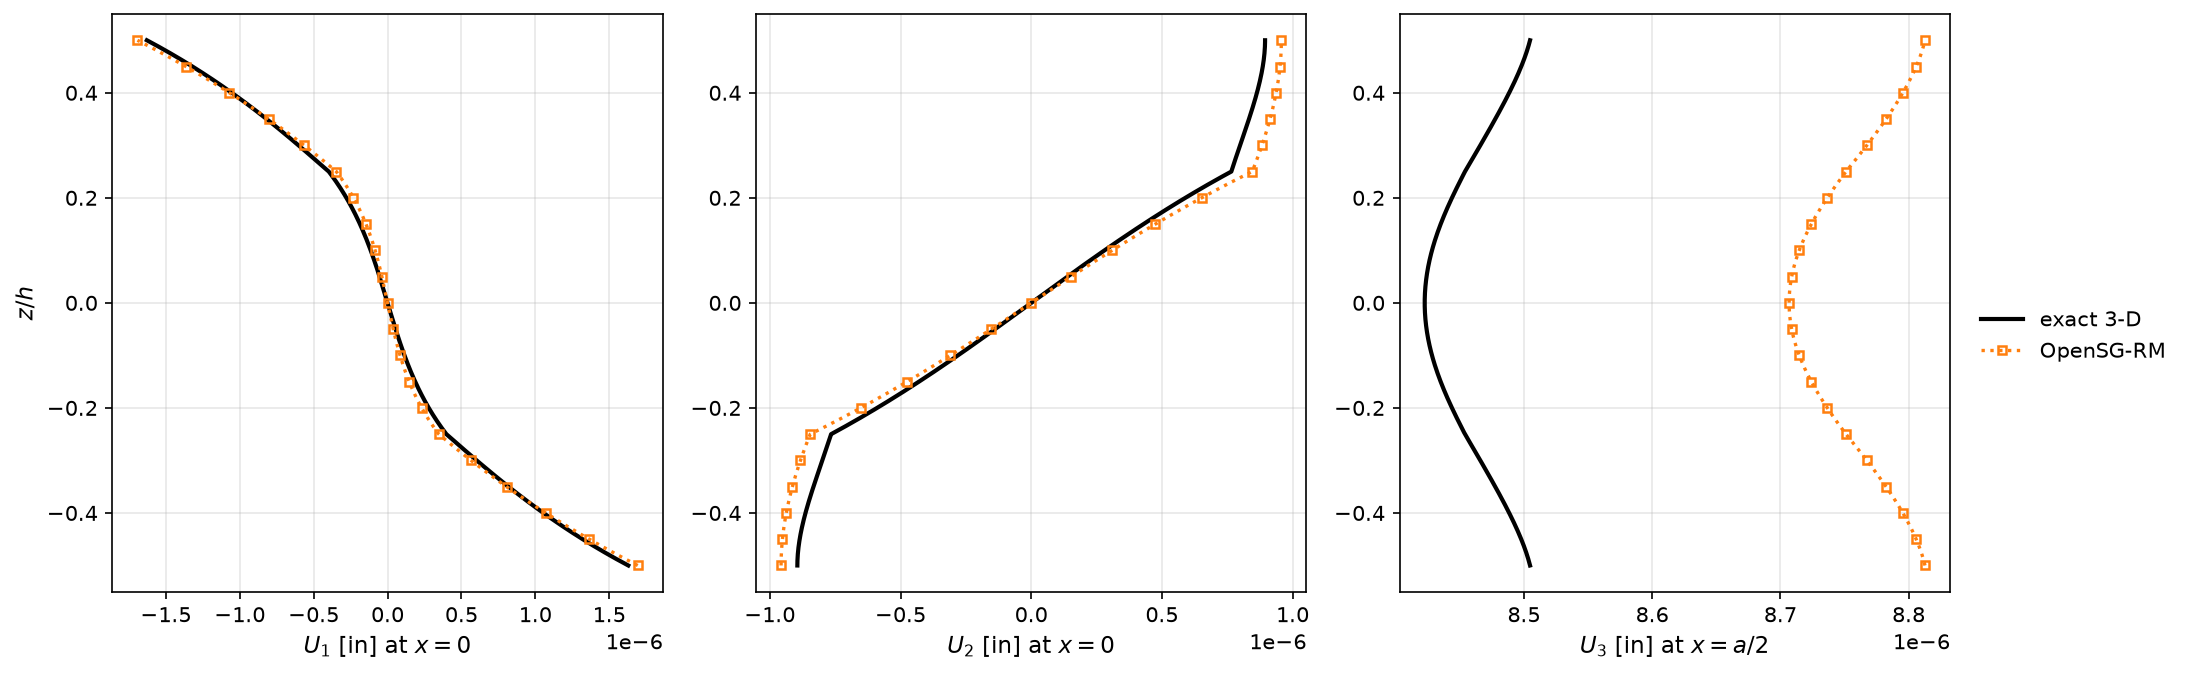
\includegraphics[width=0.98\textwidth]{tutorial_case4_disp.png}
\caption{Recovered 3-D displacements.}
\end{figure}

%=====================================================================
\newpage
\section{Reading the errors}
All four cases fall at second order in thickness: halving $h/a$ divides
every error by $\approx4$.  The $L/h=4$ numbers of Tutorials 3--4 are the
deliberately thick limit; at $S=10$ they drop to a few percent and by
$S=50$--64 to the 0.05--0.2\,\% level (the machine-generated check-value
table in the User Manual freezes the anchors).

\paragraph{The $U_2$/$U_3$ offsets of the thick cases.}
In Tutorials 3--4 the displacement \emph{shapes} follow the exact
solution while the curves sit at a small constant offset.  That offset
is the \emph{plate solution}, not the recovery: the plate displacement
is by definition the thickness average of the 3-D field, and at
$L/h{=}4$ the plate model's amplitudes differ from the exact averages
by their second-order remainder --- measured directly,
$v_{\text{plate}}$ vs $\langle U_2\rangle_{\text{exact}}$ is $-4.8\,\%$
at $L/h{=}4$ and $-0.8\,\%$ at $S{=}10$ (Tutorial 3), and
$w_{\text{plate}}$ vs $\langle U_3\rangle_{\text{exact}}$ is
$+4.5\,\%\rightarrow+2.9\,\%$ (Tutorial 3) and
$+3.5\,\%\rightarrow+0.4\,\%$ (Tutorial 4).  The recovered
through-thickness variation added on top is zero-mean by construction
and matches the exact shape.  (Tutorial 4's $U_2$ is special: the
symmetric layup has $\langle U_2\rangle=0$ identically, so its whole
profile is thickness warping --- the $9\,\%$ there is the thick-plate
shape error of the same field that gives $\sigma_{23}$ its $16\,\%$,
and it falls at the same second-order rate.)

The failure indices printed by every script use \emph{example}
allowables --- replace the \code{Xt/Xc/Yt/Yc/S12a/S13a/S23a} block with
your material system before drawing conclusions.
\end{document}
